
\documentclass[12pt]{article}

\usepackage{graphicx}
\usepackage{hyperref}
\usepackage{bibunits}
\usepackage{longtable}
\usepackage{natbib}
\usepackage{titlesec}
\hypersetup{
    colorlinks = true,
    linkcolor = {green},
}
\usepackage{verbatim}
\usepackage{lineno}

\newenvironment{instruction}{\par\color{red}}{\par}

% begin add subsubsubsection
\titleclass{\subsubsubsection}{straight}[\subsection]

\newcounter{subsubsubsection}[subsubsection]
\renewcommand\thesubsubsubsection{\thesubsubsection.\arabic{subsubsubsection}}
\renewcommand\theparagraph{\thesubsubsubsection.\arabic{paragraph}} % optional; useful if paragraphs are to be numbered

\titleformat{\subsubsubsection}
  {\normalfont\normalsize\bfseries}{\thesubsubsubsection}{1em}{}
\titlespacing*{\subsubsubsection}
{0pt}{3.25ex plus 1ex minus .2ex}{1.5ex plus .2ex}

\makeatletter
\renewcommand\paragraph{\@startsection{paragraph}{5}{\z@}%
  {3.25ex \@plus1ex \@minus.2ex}%
  {-1em}%
  {\normalfont\normalsize\bfseries}}
\renewcommand\subparagraph{\@startsection{subparagraph}{6}{\parindent}%
  {3.25ex \@plus1ex \@minus .2ex}%
  {-1em}%
  {\normalfont\normalsize\bfseries}}
\def\toclevel@subsubsubsection{4}
\def\toclevel@paragraph{5}
%\def\toclevel@paragraph{6}
\def\toclevel@subparagraph{6}
\def\l@subsubsubsection{\@dottedtocline{4}{7em}{4em}}
\def\l@paragraph{\@dottedtocline{5}{10em}{5em}}
\def\l@subparagraph{\@dottedtocline{6}{14em}{6em}}
\makeatother

\setcounter{secnumdepth}{4}
\setcounter{tocdepth}{4}
% end add subsubsubsection

\linenumbers

\title{Enabling Naturalistic, Long-Duration and Continual Experimentation with
Advanced Machine Learning Methods}

\begin{document}
\defaultbibliography{longDurationExperimentation,neuroEthology,machineLearning,signalProcessing,bonsai}
\defaultbibliographystyle{apalike}

\tableofcontents

\pagebreak

\section{Summary}


\begin{instruction}
Word limit: 550

In plain English, provide a summary we can use to identify the most suitable
experts to assess your application.

We usually make this summary publicly available on external-facing websites,
therefore do not include any confidential or sensitive information. Make it
suitable for a variety of readers, for example:

\begin{itemize}
    \item opinion-formers
    \item policymakers
    \item the public
    \item the wider research community
\end{itemize}

\paragraph{Guidance for writing a summary}

Clearly describe your proposed work in terms of:

\begin{itemize}
    \item context
    \item the challenge the project addresses
    \item aims and objectives
    \item potential applications and benefits
    \item its relevance to the
    \href{https://www.ukri.org/publications/bbsrc-strategic-delivery-plan/}{BBSRC long-term research and innovation priorities}
    and, if applicable
    \href{https://www.ukri.org/councils/bbsrc/remit-programmes-and-priorities/our-research-portfolio-and-priorities/responsive-mode-spotlights/}{Responsive Mode Spotlight areas}

\end{itemize}
\end{instruction}



\pagebreak
\section{Core team}


\begin{description}
    \item[project lead (PL)] Prof.~Maneesh Sahani
    \item[project co-lead (UK) (PcL)] Prof.~Tiago Branco, Prof.~Thomas Mrsic-Flogel
    \item[researcher co-lead (UK) (RcL)] Dr.~Joaquin Rapela, Dr.~Dario Campagner
    \item[professional enabling staff] Dr.~Adam Tyson
\end{description}


\pagebreak
\section{Application questions}

\subsection{BBSRC schemes}


\begin{instruction}
Word limit: 1

Indicate the scheme through which you are applying.

In the text box, copy the number corresponding to the scheme you are applying
through. These are:

\begin{enumerate}
    \item standard (no scheme)
    \item Industrial Partnership Award (IPA)
    \item LINK
    \item Brazil (FAPESP)
    \item Luxembourg (FNR)
    \item NSF-Bio
\end{enumerate}

Additional guidance

This is for administrative purposes to help the initial application processing.

Please follow the scheme specific guidance below and upload the additional
documents listed as a single PDF no larger than 8MB:

IPA or LINK:

\begin{itemize}

    \item a letter from your institution’s technology transfer office outlining the
management of outputs from the proposed research

\end{itemize}

FAPESP:

\begin{itemize}

    \item FAPESP proposal form
    \item FAPESP consolidated budget form
    \item FAPESP letter of eligibility

\end{itemize}

FNR:

\begin{itemize}

    \item CVs of international collaborators
    \item FNR ‘INTER’ budget form
    \item FNR ‘INTER’ cost justification

\end{itemize}

NSF-Bio:

\begin{itemize}

    \item US biosketches
    \item US budget forms

\end{itemize}
\end{instruction}


\pagebreak
\subsection{BBSRC remit classification}


\begin{instruction}
Word limit: 1

Your application will be considered by one of our four research committees
made up of independent experts. Indicate which you feel would be best placed
to assess your application.

In the text box, write only the letter (in uppercase) corresponding to the
committee you feel would be best placed to assess your application. These are:

\begin{description}

    \item[A] animal disease, health and welfare

    \item[B] plants, microbes, food and sustainability

    \item[C] genes, development, and science, technology, engineering and maths
    (STEM) approaches to biology

    \item[D] molecules, cells and industrial biotechnology

\end{description}

Additional guidance:

This is for administrative purposes to help the initial application processing.
We will check your choice and make a final decision as to which committee will
assess your application.

\end{instruction}


\pagebreak
\subsection{Vision}
\begin{instruction}
Word limit: 550

What are you hoping to achieve with your proposed work?

What the assessors are looking for in your response

Explain how your proposed work:

\begin{enumerate}

    \item is of excellent quality and importance within or beyond the field(s) or area(s)

    \item has the potential to advance current understanding, or generate new
knowledge, thinking or discovery within or beyond the field or area

    \item is timely given current trends, context, and needs

    \item impacts world-leading research, society, the economy, or the environment

\end{enumerate}

You may demonstrate elements of your responses in visual form if relevant.
Further details are provided in the Funding Service.
References may be included within this section.
\end{instruction}

\begin{bibunit}
\subsection{Context}

Conventional systems neuroscience experiments are typically short in duration
and often place significant constraints on subject behavior to simplify data
analysis.
%
However, these restrictions may limit our ability to observe critical
aspects of brain function and behavior that only manifest in more naturalistic
and extended conditions.

At the Sainsbury Wellcome Centre (SWC) for Neural Circuits and Behaviour, we
are pioneering Naturalistic, Long-Duration, and Continual (NaLoDuCo) foraging
experiments in mice that span weeks to months. During these extended
experiments, we collect high-resolution recordings of both behavioral and
neural activity in naturalistic settings.
%
In collaboration with the Gatsby Computational Neuroscience Unit (GCNU), we are
developing novel analytical methods to interpret this new class of data.

This novel experimental approach will enable researchers to explore neural
mechanisms underlying behavior over extended periods for the first time,
offering the possibility of uncovering insights across a wide range of
phenomena, including long-term behavioral adaptation, neural plasticity, and
learning.
%
The data generated from NaLoDuCo experiments represent an entirely
new resource in neuroscience, with the potential to drive breakthroughs and
discoveries that are beyond the reach of traditional experiments.

Our vision is to empower research centers worldwide to adopt this
groundbreaking approach.
%
However, the scale and complexity of the data generated pose significant
challenges in data acquisition, visualisation, and analysis.
%
In this proposal, we will address these challenges, developing and sharing
openly the necessary expertise, hardware, and software to enable this
transformative type of experimentation on a global scale.

\subsection{Focus areas and their challenges}

Below, we outline the key focus areas we aim to address
(Figure~\ref{fig:focusAreas}), along with their associated challenges.
%
These challenges primarily revolve around the collection and analysis of
continuously recorded, extremely large datasets--on the order of hundreds of
terabytes--gathered from experiments spanning weeks to months.

While experiments in neuroscience that are naturalistic, long-duration, or
continuous have been conducted in the past
\citep[e.g.,][]{jhuangEtAl10,maoEtAl21,volohEtAl23}, to the best of our
knowledge, we are the first to integrate all three of these features in a
single experimental paradigm.
%
This combination introduces unprecedented complexities in data processing, as
we aim to capture behavior and brain activity in their most ecologically valid,
extended, and uninterrupted forms.

\begin{figure}
    \begin{center}
        \resizebox{4.0in}{!}{%
            \resizebox{5in}{!}{%
    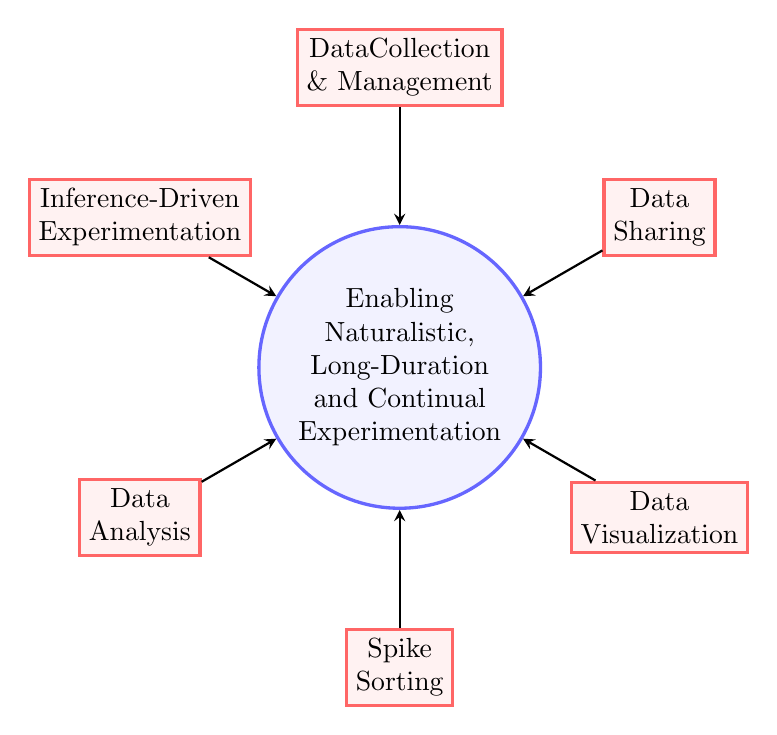
\begin{tikzpicture}[
            node distance=4cm and 1cm,
            centralNode/.style={circle, draw=blue!60, fill=blue!5, very thick,
            minimum size=7mm, align=center},
            itemNode/.style={rectangle, draw=red!60, fill=red!5, very thick,
            minimum size=5mm, align=center},
            arrow/.style={thick, <-, >=stealth},
        ]
        \node[centralNode] (naloducoExp)    {Enabling\\Naturalistic,\\Long-Duration\\and Continual\\Experimentation};
        % \node[itemNode]    (dataCol)        at (naloducoExp) ++(40:2cm) {DataCollection\\\& Management};
            \path (naloducoExp) ++(90:1.5in) node[itemNode] (dataCol) {DataCollection\\\& Management};
            \path (naloducoExp) ++(30:1.5in) node[itemNode] (dataSharing) {Data\\Sharing};
            \path (naloducoExp) ++(330:1.5in) node[itemNode] (dataVis) {Data\\Visualization};
            \path (naloducoExp) ++(270:1.5in) node[itemNode] (spikeSort) {Spike\\Sorting};
            \path (naloducoExp) ++(210:1.5in) node[itemNode] (dataAnalysis) {Data\\Analysis};
            \path (naloducoExp) ++(150:1.5in) node[itemNode] (inferenceDExp) {Inference-Driven\\Experimentation};
        \draw[arrow] (naloducoExp) -- (dataCol);
        \draw[arrow] (naloducoExp) -- (dataSharing);
        \draw[arrow] (naloducoExp) -- (dataVis);
        \draw[arrow] (naloducoExp) -- (spikeSort);
        \draw[arrow] (naloducoExp) -- (dataAnalysis);
        \draw[arrow] (naloducoExp) -- (inferenceDExp);
    \end{tikzpicture}
}

        }
    \end{center}
    \caption{Project theme (blue) and focus areas (red).}
    \label{fig:focusAreas}
\end{figure}

\subsubsection{Data acquisition and management}

At the SWC we have already performed foraging experiments in mice continuously collecting
behavioral and experimental data 24 hours a day for seven days.
%
We will share openly the specifications of the hardware used to build these
experiments (e.g., instructions for building large foraging arenas, video
cameras specifications, electrophysiological recording hardware), as well as
the software we used for experimental control, data quality control, data
access and management.

The data acquisition and management software used in our project is already
publically available in
GitHub\footnote{\url{https://github.com/SainsburyWellcomeCentre/aeon\_mecha}}.
%
This software is already being used by scientists at the Allen Institue for
Neural Dynamics and at Northwester University.
%
We will substantially improve its documentation to simplify its usage by
external users.

Challenges related to data acquisition and management include data indexing to
allow fast access to very large amount of saved data, online quality control
and alert systems to guarantee that anomalities in data collection are detected
and corrected with minimal delay, and syncrhonization between multiple data
streams.

\subsubsection{Data dissemination}

Datasets of the scale of hundreads of terabytes cannot be practically
downloaded from data repositories. This is specially true for contiguous
experiments where unique insights are extracted by characterizing full
datasets, and not only parts of them.
%
Therefore, we will store data in DANDI, which uses Amazon S3 buckets, and
provide software in Amazon EC2 instances to visualize and analyze data on the
cloud, avoiding costly data transfers.
%
That is, the large dataset sizes of NaLoDuCo experiments make it impractical to
distribute data to users and require to bring users to data.
%
Fortunately, cloud technologies are now mature to allows this.

Importantly, if we distributed these very large datasets to users, only those
in large research centers would have the computing power to process them. But, by deploying data
and computing in the cloud, any person with Internet access around the world
will be able to benefit from them.
%
Storing large datasets in DANDI is free.
% and it is possible to obtain cloud credits from Amazon to offer free compute to academic institution.

Dr.~Ben Ditcher, founder of CatalystNeuro, has played a pivotal role in
supporting the development and operations of the DANDI archive.

\subsubsection{Data visualisation}

Visualisations are essential for scientific discovery.
%
For the proposed project visualisation present two major challenges. First, they need
to display very large datasets at different temporal scales, from milliseconds
to weeks and months. Second, as data and software will be deployed in the
cloud, visualisation need to be web based.
%
Standard visualization tools cannot display terabyte sized datasets.
%
We will build custom web-based visualization tools to do this.

We have substantial experience building web-based visualization tools for
neurophysiological data. Dr.~Jeremy Magland is now developing
Neurosift\footnote{\url{https://github.com/flatironinstitute/neurosift}} a web-based
visualizer for DANDI datasets.

\subsubsection{Spike sorting}

When electrodes are placed in the brain, they typically record spikes from
multiple nearby neurons. Spike sorting attributes spikes to individual neurons.

Spike sorting is specially challenging for NaLoDuCo experiments.
%
First, because these experiments require to track individual neurons of freely
moving mice for weeks to months.
%
Second, because spike sorting needs to be done online, to allow experiments
driven by real-time machine learning inference, as described below.

Prof.~Sahani pioneered the use of Bayesian inference methods for spike
sorting~\citep{sahani99}.
%
Dr.~Jeremy Magland has significantly advanced the field of spike sorting,
particularly through his development of
MountainSort\footnote{\url{https://github.com/flatironinstitute/mountainsort5}}
and his contributions to
SpikeInterface\footnote{\url{https://github.com/spikeinterface/spikeinterface}}.

\subsubsection{Data analysis}

Advanced data analysis methods are indispensable to extract meaning from
NaLoDuCo experimental data.
%
However, analyzing this data is challenging for at least three reasons.
%
First, important insights will most probably come from the characterization of
complete datasets, and not form subsets extracted from them. Conventional batch
methods cannot be used with datasets of the size produced by NaLoDuCo
experiments.
%
For instance, for learning, batch linear regression cannot load into memory and
invert a data matrix with high-resolution observations from a one-month-long
experiment.
%
Thus, \textbf{online methods} that can process infinite data steams become
mandatory.

Second, a pervasive assumption in most ML algorithms is stationarity; i.e., the
assumption that the statistics of data do not change over time.
%
But in long-duration and continuous experiments this assumption is most often
violated as, for example, the arousal of subjects changes.
%
Hence, the analysis of data generated by these experiments requires
\textbf{adaptive methods}.

Third, statistical algorithms consist of two key stages: learning (or
trainning) and inference (or prediction). The learning stage identifies model
parameters, and the inference stage uses the learned model to make predictions,
or infer latent variables, from new unseen data.
%
Frequently training is performed on a small subset of a dataset, and inference
is done on the remaining data.  However, since in long-duration and continual
experiments behavior and neural activity are generall not stationary, it is not
optimal to train models on data subsets and use them to make inferences on the
remaining data, since the state of the animal at training and inference times
may be different.
%
To overcome this difficulty we will use \textbf{continual learning methods}.

We will evaluate methods to analyze different aspects of behavior and neural
activity (Figure~\ref{fig:dataAnalysisFocus}).
%
We will test how these methods process very large datasets, how they handle
non-stationary data, and how feasible is to retrain them to adapt to
changing conditions.
%
We will adapt these methods so that they better address these challenges and,
when needed, develop new ones.
%
We will carefully report the outcomes of these evaluations so that researchers
performing NaLoDuCo experimentation can choose the best methods that suit their
needs.

\subsubsection{Experiments driven by real-time machine learning inference}

Small animal experiments are usually controlled by simple static rules or
direct behavioral observations.
%
Funded by a BBSRC
award\footnote{\url{https://gow.bbsrc.ukri.org/grants/AwardDetails.aspx?FundingReference=BB\%2FW019132\%2F1}}
we are developing software to allow a new type of experimental control based on
statistical inferences made on behavioral and/or neural measurements.

For example, after inferring latent variables from neural activity and
observing that one of these latents have crossed a threshold, we can
deliver a reward \citep[as done in learning to control a
BCI;][]{clancyAndMrsicFlogel21}, or perform an action~\citep[as done in motor imagery
BCI;][]{lebedevAndNicolelis06}, or manipulate of neural activity~\citep[as
done when studying the causal relation between a pattern of brain activity and
behavior;][]{deisseroth15}.
%
We propose to further develop the previous software and use it to test causal
effects of neural activity patterns on foraging decisions using our NaLoDuCo
foraging experiments.

Buidling experiments driven by real-time machine learning inferences brings at
least two challenges. The first one is a machine learning problem, how to build
fast inferences that can operate in real time. The second one is a neuroscience
problem, how to identify neuroscience experiments suitable to real-time
control, and then perform the experiment with real-time control.
%
Fortunately at the Gatsby Unit we are experienced on building advanced machine
learning algorithms to address the first challenge. And at the SWC we perform
many sophisticated animal experiments that could benefit from real-time
experimental control.

In summary, we are pioneering a new paradigm in neuroscience experimentation,
driven by advanced inferential methods applied to rich behavioral and neural
recordings. This innovative technology has the potential to transform the
field, enabling experiments that were previously unimaginable. By leveraging
these sophisticated inferences, we may unlock new dimensions of knowledge that
could not be achieved through simpler, conventional approaches. This
breakthrough could open doors to insights that redefine our understanding of
brain-behavior relationships.



\putbib
\end{bibunit}

\pagebreak
\subsection{Approach}

\begin{instruction}

Word limit: 3,300

How are you going to deliver your proposed work?

What the assessors are looking for in your response

Explain how you have designed your approach so that it:

\begin{enumerate}

    \item is effective and appropriate to achieve your objectives

    \item is feasible, and comprehensively identifies any risks to delivery and
    how they will be managed

    \item uses a clearly written and transparent methodology (if applicable)

    \item summarises the previous work and describes how this will be built
    upon and progressed (if applicable)

    \item will maximise translation of outputs into outcomes and impacts

    \item describes how your, and if applicable your team’s, research
    environment (in terms of the place and relevance to the project) will
    contribute to the success of the work

\end{enumerate}

You may demonstrate elements of your responses in visual form if relevant.

Please make sure to check sizing and readability of the image using ‘read view’
prior to submission. Further details are provided in the Funding Service.

References may be included within this section.

Within the ‘Approach’ section we also expect you to:

\begin{itemize}

    \item provide a detailed and comprehensive project plan including
    milestones and timelines in the form of an embedded Gantt chart or similar
    (please make sure to check sizing and readability of the image using ‘read
    view’ prior to submission)

\end{itemize}

BBSRC’s
\href{https://www.ukri.org/publications/bbsrc-equality-diversity-and-inclusion-action-plan/bbsrc-action-plan-for-equality-diversity-and-inclusion-in-the-biosciences-2022-to-2025/}{action
plan for EDI} outlines our commitment to removing barriers to participation in
our programmes, ensuring investments do not inadvertently prevent access or
usage by individuals from minority groups, for example disabled researchers.

To this end, applications should identify how accessibility and inclusiveness
in the widest sense have been incorporated into the design of the project. For
example, you may wish to reference relevant institutional strategies and
policies which support equality, diversity, and inclusion as they relate to
access to equipment and facilities and indicate how the proposed project has
been designed and will be delivered with broad access in mind.

\end{instruction}

\begin{bibunit}
\subsubsection{Data collection \& management}

We have developed a new platform that allows housing of mice in large arenas
(\textgreater 2m diameter), while manipulating and monitoring their behaviour
at high spatiotemporal resolution \citep[Figure~\ref{fig:arena}, ][]{campagnerEtAl24}.
%
We have openly shared software for supporting data acquistion
\citep{aeonacquisition} and management \citep{aeonmecha} in this
arena.
%
Using this platform we have collected several week long datasets both with
single mouse and multiple mice.


\begin{figure}
    \centering
    \subfloat[]{
        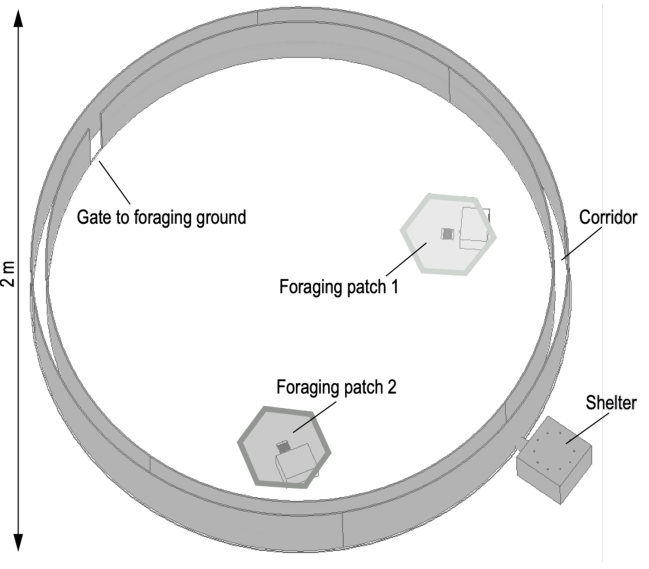
\includegraphics[width=4in]{figures/arena.png}
    }
    \hfill
    \subfloat[]{
        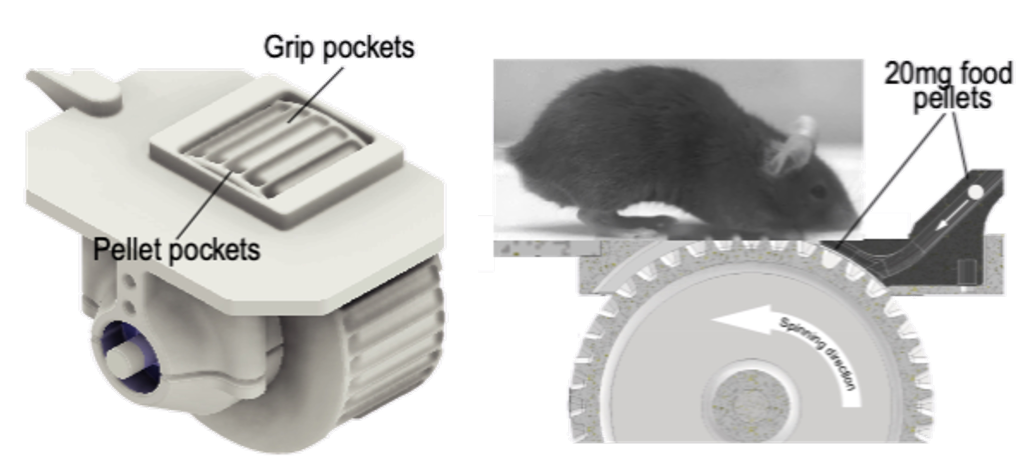
\includegraphics[width=4in]{figures/patch.png}
    }
    \caption{Foraging Arena (a) and Feeder (b).
    %
    The arena is composed of tessellated hexagonal tiles (a), each featuring a
    newly designed underground feeder (b).
    %
    Pellets are dispensed onto a foraging wheel once the mouse has spun it for
    a pre-defined programmable distance threshold using its forepaws (fictive
    digging).
    %
    The arena contains up to six scale-equipped nesting modules that allows
    housing of mice in the arena and weight monitoring.
    %
    Behavioural monitoring is achieved by an array of high-speed cameras (up to
    15), by which mouse location, mouse identity and body parts can be track in
    real time.
    %
    }
\label{fig:arena}
\end{figure}


\subsubsection{Data sharing}

The large dataset sizes generated by NaLoDuCo experiments, on the order of
hundreads of terabytes,  make it impractical to distribute data to users, and
require to bring users to data. Fortunately, cloud technologies are now mature
to allows this.
%
We will store data in the Distributed Archives for Neuroscience Data
Integration (DANDI), which uses Amazon S3 buckets, and we will provide software
to visualize and analyze data in Amazon EC2 instances, to avoid costly data
transfers.

\subsubsection{Data visualisation}

Our visualisation tools
need to display very large datasets at different temporal scales, from
milliseconds to weeks and months, and they need to be web based.
%
We will use multi-resolution visualization techniques, which store data at
various resolutions, and use the approriate resolution for each zoom level.
%
Web-based visualisation will be optimized using web workers
\citep{webWorkers}.

\subsubsection{Spike sorting}

Spike sorting is specially challenging in NaLoDuCo experimentation since we
want to track individual neurons of freely moving mice for weeks to months.
%
In addition, we need online spike sorting, to allow experiments driven
by real-time machine learning inference, as described below.

We will evaluate methods for tracking neurons over long periods of time
\citep[e.g.,][]{yuanEtAl24,vanBeestEtAl24} and for online sorting
\citep[e.g.,][]{rutishauserEtAl06,santhanamEtAl04}.

\subsubsection{Data analysis}

The very large size of NaLoDuCo experimental data, the fact that the statistics
of these data change across time, and the requirement for real-time and
close-loop inference create new challenges to conventional machine learning
methods.
%
We will evaluate existing methods targeting the experimental problems
in Figure~\ref{fig:dataAnalysis} and, if necessary, modify them, or create new
ones, to address the previous challenges.

For behavioral data, we will evaluate methods to:

\begin{itemize}

    \item track multiple body parts of
animals \citep[e.g.,][and a switching-linear-dyanamical method using RFIDs that
we will develop]{mathisEtAl18,pereiraEtAl22,bidermanEtAl24},

    \item infer kinematics of foraging mice \citep[e.g.,][]{ldspython,challaEtAl11},

    \item segment behavior into discrete states \citep[e.g.,][and a hierarchical HMM
that we will develop]{wiltschkoEtAl15,hsuAndYttri21},

    \item infer the rules that govern mice behavior from behavioral observations
only (i.e., policy inference) \citep[e.g.,][]{ziebartEtAl08,zhuEtAl23}.

\end{itemize}

For neural data, we will evaluate methods to:

\begin{itemize}

    \item estimate low-dimensional continual representations of
        high-dimensional spiking activity (i.e., latents inference)
        \citep[e.g.,][]{mackeEtAl11,dunckerAndSahani18,pandarinathEtAl18,saniEtAl21},

    \item segment neural activity into discrete states
        \citep[e.g.,][]{chenEtAl09,escolaEtAl11},

    \item decode environment variables from neural activity
        \citep[e.g.,][]{dengEtAl15,kloostermanEtAl14,tampuuEtAl19}.

\end{itemize}


\subsubsection{Inference-driven experimentation}

We call inference-driven experimentation to a type of experimentation driven by
machine learning inferences on neural or behavioral data, where the result of
these inferences can change the experiment in real time.

We will apply inference-driven experimentation to test if patterns of neural
activity are causally related to foraging behaviors.
%
We would first check that a pattern of neural activity always precedes a given
foraging behavior. We would then detect the occurence of the pattern and in
real time optogenetically inactivate the neurons responsible for the pattern.
%
If the behavior dissapears the causality argument would be supported.

For this we will use the Bonsai ecosystem for experimental
control~\citep{bonsai} and online machine learning functionality that we are
adding to Bonsai~\citep{bonsaiML}, funded by a BBSRC award~\citep{bbsrcAward}.


\putbib
\end{bibunit}

\pagebreak
\subsection{Applicant and team capability to deliver}


\begin{instruction}
Word limit: 1,650

Why are you the right individual or team to successfully deliver the proposed
work?

What the assessors are looking for in your response

Please ensure the current job titles of the core team members are included
here to ensure eligibility can be established for the core team roles assigned.
Find out more about
\href{https://www.ukri.org/publications/roles-in-funding-applications/roles-in-funding-applications-eligibility-responsibilities-and-costings-guidance/}{UKRI’s
core team roles in funding applications} and our
\href{https://www.ukri.org/councils/bbsrc/guidance-for-applicants/check-if-youre-eligible-for-funding/applicants-and-co-applicants/}{eligibility
guidance}.

Evidence of how you, and if relevant your team, have:

\begin{itemize}

    \item the relevant experience (appropriate to career stage) to deliver the proposed
work

    \item the right balance of skills and expertise to cover the proposed work

    \item the appropriate leadership and management skills to deliver the work and
your approach to develop others

    \item contributed to developing a positive research environment and wider
community

\end{itemize}

You may demonstrate elements of your responses in visual form if relevant.

Further details are provided in the Funding Service.

The word limit for this section is 1,650 words: 1,150 words to be used for R4RI
modules (including references) and, if necessary, a further 500 words for
Additions.

Use the Résumé for Research and Innovation (R4RI) format to showcase the range
of relevant skills you and, if relevant, your team (project and project
co-leads, researchers, technicians, specialists, partners and so on) have and
how this will help deliver the proposed work. You can include individuals’
specific achievements but only choose past contributions that best evidence
their ability to deliver this work.

Complete this section using the R4RI module headings listed. Use each
heading once and include a response for the whole team, see the UKRI
guidance on R4RI. You should consider how to balance your answer, and
emphasise where appropriate the key skills each team member brings:

\begin{itemize}

    \item contributions to the generation of new ideas, tools, methodologies, or
knowledge

    \item the development of others and maintenance of effective working relationships

    \item contributions to the wider research and innovation community

    \item contributions to broader research or innovation users and audiences and
towards wider societal benefit

\end{itemize}

Additions

Provide any further details relevant to your application. This section is
optional and can be up to 500 words. You should not use it to describe
additional skills, experiences, or outputs, but you can use it to describe any
factors that provide context for the rest of your R4RI (for example, details of
career breaks if you wish to disclose them).

Complete this as a narrative. Do not format it like a CV.

References may be included within this section.

The roles in funding applications policy has descriptions of the different
project roles.

\end{instruction}


\pagebreak
\subsection{Project partners}


\begin{instruction}

Add details about any project partners’ contributions. If there are no project
partners, you can indicate this on the Funding Service.

A project partner is a collaborating organisation who will have an integral
role in the proposed research. This may include direct (cash) or indirect
(in-kind) contributions such as expertise, staff time or use of facilities.
Project partners may be in industry, academia, third sector or government
organisations in the UK or overseas, including partners based in the EU.

If you are applying via the IPA or LINK scheme, please include details of
industry partners here.

If applying under the BBSRC-NSF lead agency scheme, please include details
of your US partner here.

Add the following project partner details:

\begin{itemize}

    \item the organisation name and address (searchable via a drop-down list or enter
the organisation’s details manually, as applicable)

    \item the project partner contact name and email address

    \item the type of contribution (direct or in-direct) and its monetary value
\end{itemize}

If a detail is entered incorrectly and you have saved the entry, remove the
specific project partner record and re-add it with the correct information.

For audit purposes, UKRI requires formal collaboration agreements to be put in
place if an award is made.

\end{instruction}


\pagebreak
\subsection{Project partners: statement of support}

\begin{instruction}

Word limit: 3,000

Only complete a statement of support if you have named project partners in the
project partner section above. A statement is required to be provided from each
partner you named in the ‘Project partners’ section.

If you are applying via the IPA or LINK scheme, please include details of
industry partner support here.

What the assessors are looking for in your response

A project partner is a collaborating organisation who will have an integral
role in
the proposed research. This may include direct (cash) or indirect (in-kind)
contributions such as expertise, staff time or use of facilities.

Each statement should:

\begin{itemize}

    \item confirm the partner’s commitment to the project

    \item clearly explain the value, relevance, and possible benefits of the
    work to them

    \item describe any additional value that they bring to the project

\end{itemize}

Ensure you have prior agreement from project partners so that, if you are
offered funding, they will support your project as indicated in the ‘Project
partners’ section.

For audit purposes, UKRI requires formal collaboration agreements to be put in
place if an award is made.

Do not provide a statement of support from host and project co-leads’ research
organisations.

Do not provide a statement of support from collaborators. Contributions from
collaborators not listed as project partners can be outlined in ‘Applicant and
team capability to deliver’.

\end{instruction}


\end{document}
